\begin{surferPage}[莱布斯7次曲面]{莱布斯7次曲面}
2004年,奥利弗莱布斯在美因茨大学完成他的学位论文时构造了一个7次曲面。这是7次曲面的当今世界纪录。但是,仍然
有可能存在104个奇异点的7次曲面。  莱布斯的曲面具有正7边形(左图)的对称性。这可以从曲面的顶部观察到(右图)

    \vspace*{-0.3em}
    \begin{center}
      \begin{tabular}{c@{\qquad}c}
        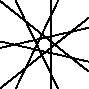
\includegraphics[height=1.5cm]{./../../common/images/labsseptic1.pdf}
        &
        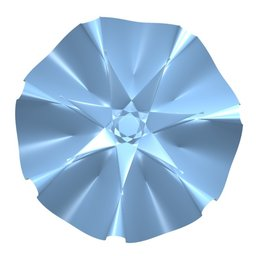
\includegraphics[height=1.5cm]{./../../common/images/labs_septic_von_oben}
      \end{tabular}
    \end{center}
    \vspace*{-0.3em}

为了构造这个曲面,奥利弗莱布斯利用了计算代数几何以及奇异点中流行的计算机系统{\sc Singular}(凯撒斯劳滕大学)。
我们知道时钟的规则是:24.00$=$0.00, 24.00 $+$ 1 小时是1点,而不是25点。这种有限集上的自然计算规则同样被奥利弗莱布斯加以利用。
\end{surferPage}
